% The ID is the innermost part of the ATLAS detector and measures the direction, momentum, and charge of charged particles produced in the proton-proton collision. When charged particles travel away from the interaction point (IP), they deposit energy in the sub-detectors of the ID, which are referred to as hits. These hits are then used to reconstruct the trajectory, referred to as tracks, of the particle via track reconstruction. This allows the charge and momentum of particles to be determined. Due to a large influx of particles during the proton-proton collision, the ID is designed to make high-precision measurements because of its high granularity. 

% As mentioned in Section~\ref{sec:atlas_magnet}, the ID is surrounded by the superconducting solenoid, which provides a uniform 2~T magnetic field inside of the ID\@. This allows particles to curve and give the required information needed for track reconstruction. The ID only reconstructs charged particles whose momentum in the transverse plane (\pt) is above 500 MeV and within the pseudorapidity range of $|\eta| < 2.5$. The ID can be seen in Figure~\ref{fig:atlas_id}.

% \begin{figure}
%     \centering
%     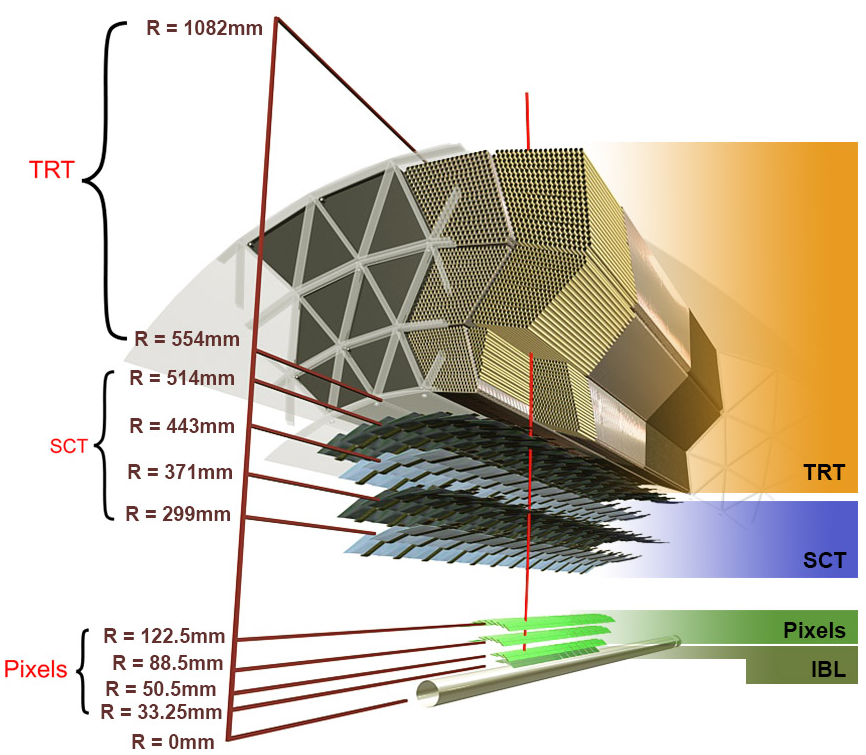
\includegraphics[width=0.8\textwidth]{figures/atlas/atlas_ID.png}
%     \caption{A cross sectional view of the barrel region of the ID is shown. Depicted is a particle originating from the IP traversing through the four layers of the pixel detector, through the SCT and finally through many TRT straws. Taken from~\cite{atlas_inner_detector_image}}\label{fig:atlas_id}
% \end{figure}

% \begin{figure}
%     \centering
%     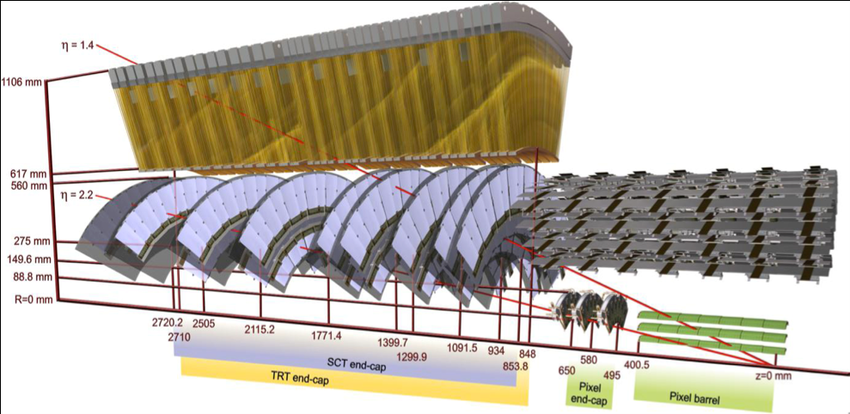
\includegraphics[width=0.8\textwidth]{figures/atlas/atlas_ID_endcap.png}
%     \caption{A schematic of the ID end-cap detectors with several red lines drawn at different $\eta$ values, demonstrating a particle traversing through the detector. Additionally, this schematic shows all of the different detector technologies in the end-cap region. Taken from~\cite{atlas_inner_detector_endcap_image}}\label{fig:atlas_id_endcap}
% \end{figure}

%%%%%%%%%%%%%% revision
The ID is the innermost part of ATLAS and measures the charge, momentum, and direction of charged particles produced in the $pp$ collisions. As charged particles pass through the ID they deposit energy in the detector and those deposits are then used in track reconstruction to infer their trajectories. Even with a high influx of particles during the $pp$ collision, the ID makes precise measurements due to its high granularity.

As mentioned previously, the ID is surrounded by the superconducting solenoid which provides a uniform 2~T magnetic field inside of the ID\@. This magnetic field bends the particles trajectories and allows for precision momentum measurements as the ID only reconstructs charged particles whose momentum in the transverse plane (\pt) is above 500 MeV and within the pseudorapidity range of $|\eta| < 2.5$. The ID can be seen in Figure~\ref{fig:atlas_id}.

\begin{figure}
    \centering
    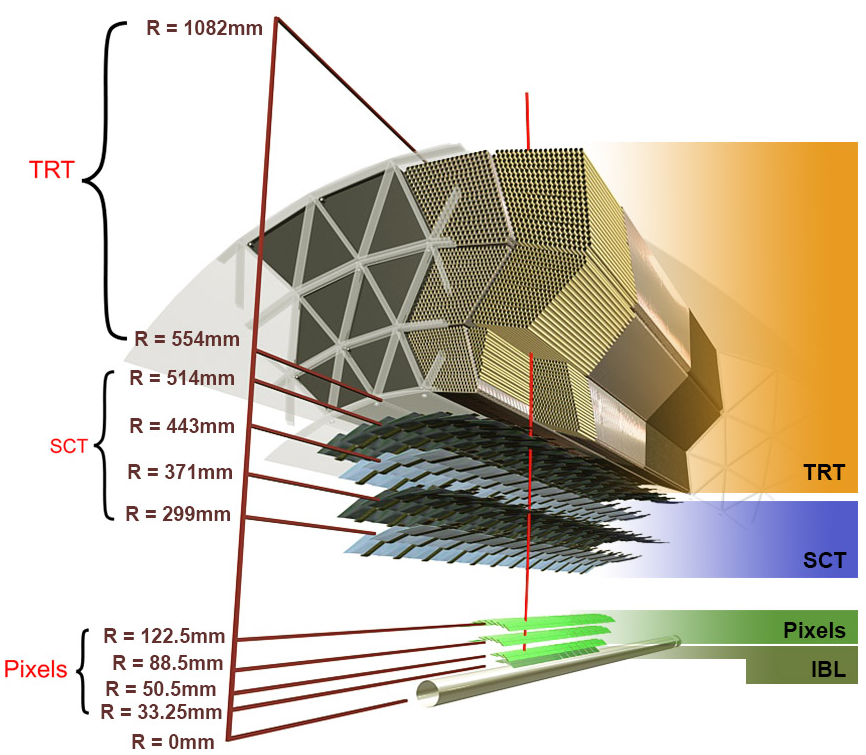
\includegraphics[width=0.8\textwidth]{figures/atlas/atlas_ID.png}
    \caption{A cross sectional view of the barrel region of the ID is shown. Depicted is a particle originating from the IP traversing through the four layers of the pixel detector, through the SCT and finally through many TRT straws. Taken from~\cite{atlas_inner_detector_image}}\label{fig:atlas_id}
\end{figure}

\begin{figure}
    \centering
    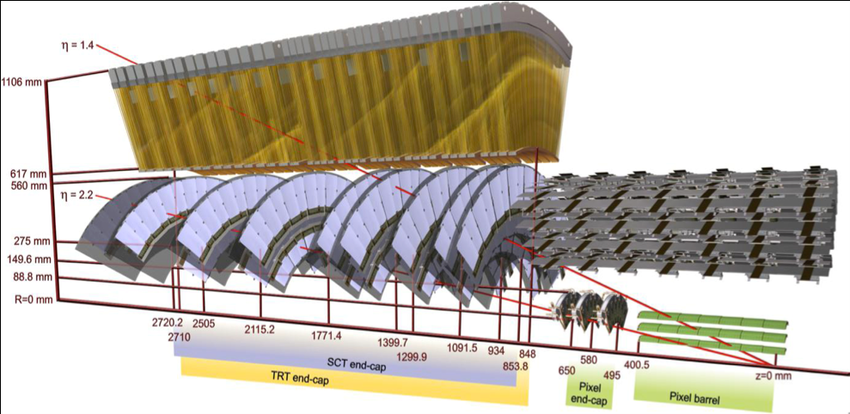
\includegraphics[width=0.8\textwidth]{figures/atlas/atlas_ID_endcap.png}
    \caption{A schematic of the ID end-cap detectors with several red lines drawn at different $\eta$ values, demonstrating a particle traversing through the detector. Additionally, this schematic shows all of the different detector technologies in the end-cap region. Taken from~\cite{atlas_inner_detector_endcap_image}}\label{fig:atlas_id_endcap}
\end{figure}
